\documentclass{ximera}


\graphicspath{
  {./}
  {ximeraTutorial/}
  {basicPhilosophy/}
}

\newcommand{\mooculus}{\textsf{\textbf{MOOC}\textnormal{\textsf{ULUS}}}}

\usepackage{tkz-euclide}\usepackage{tikz}
\usepackage{tikz-cd}
\usetikzlibrary{arrows}
\tikzset{>=stealth,commutative diagrams/.cd,
  arrow style=tikz,diagrams={>=stealth}} %% cool arrow head
\tikzset{shorten <>/.style={ shorten >=#1, shorten <=#1 } } %% allows shorter vectors

\usetikzlibrary{backgrounds} %% for boxes around graphs
\usetikzlibrary{shapes,positioning}  %% Clouds and stars
\usetikzlibrary{matrix} %% for matrix
\usepgfplotslibrary{polar} %% for polar plots
\usepgfplotslibrary{fillbetween} %% to shade area between curves in TikZ
\usetkzobj{all}
\usepackage[makeroom]{cancel} %% for strike outs
%\usepackage{mathtools} %% for pretty underbrace % Breaks Ximera
%\usepackage{multicol}
\usepackage{pgffor} %% required for integral for loops



%% http://tex.stackexchange.com/questions/66490/drawing-a-tikz-arc-specifying-the-center
%% Draws beach ball
\tikzset{pics/carc/.style args={#1:#2:#3}{code={\draw[pic actions] (#1:#3) arc(#1:#2:#3);}}}



\usepackage{array}
\setlength{\extrarowheight}{+.1cm}
\newdimen\digitwidth
\settowidth\digitwidth{9}
\def\divrule#1#2{
\noalign{\moveright#1\digitwidth
\vbox{\hrule width#2\digitwidth}}}






\DeclareMathOperator{\arccot}{arccot}
\DeclareMathOperator{\arcsec}{arcsec}
\DeclareMathOperator{\arccsc}{arccsc}

















%%This is to help with formatting on future title pages.
\newenvironment{sectionOutcomes}{}{}


\author{Lee Wayand}

\begin{document}
\begin{exercise}  





Below is the graph of $z=g(t)$.  

\begin{image}
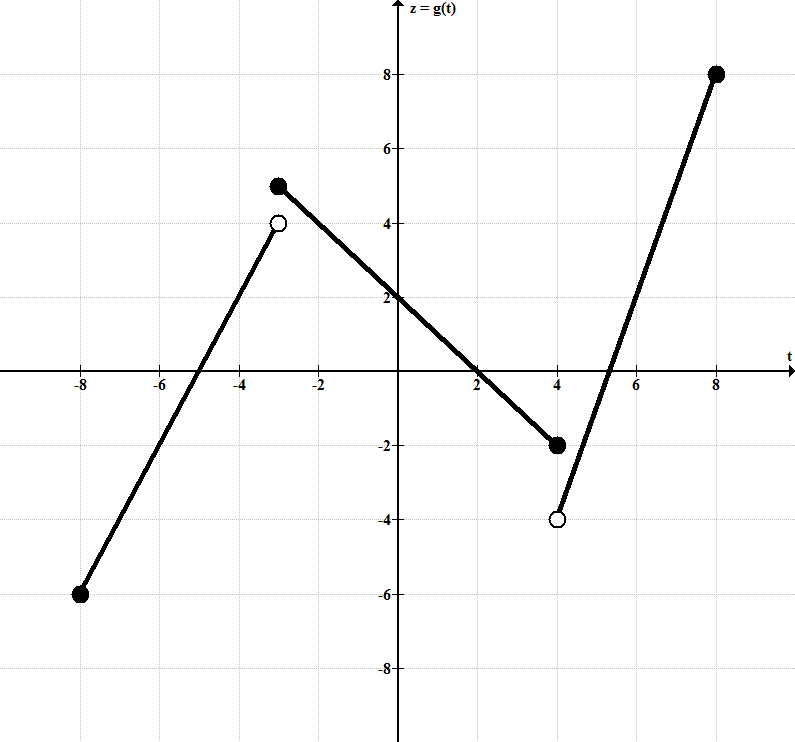
\includegraphics{../../pics/func_graphs/f30.png}
\end{image}


\begin{question} 

What is the domain of $g$?


\begin{multipleChoice}
\choice {$[-8, -3) \cup (-3, 4) \cup (4, 8)$}
\choice {$[-6, 8)$}
\choice {$(-\infty, \infty)$}
\choice {$[-8, 8]$}

\end{multipleChoice}

\end{question}





\begin{question} 






Evaluate $g(-8) = \answer[tolerance=0.25]{-6}$


Classify $4$. \\


\begin{multipleChoice}
\choice {Discontinuity}
\choice {Singularity}
\choice [correct]{Neither}
\end{multipleChoice}





Evaluate $g(-3) = \answer[tolerance=0.25]{5}$


Classify $-3$. \\


\begin{multipleChoice}
\choice [correct]{Discontinuity}
\choice {Singularity}
\choice {Neither}
\end{multipleChoice}





Evaluate $g(4) = \answer[tolerance=0.25]{-2}$


Classify $4$. \\


\begin{multipleChoice}
\choice [correct]{Discontinuity}
\choice {Singularity}
\choice {Neither}
\end{multipleChoice}




Evaluate $g(8) = \answer[tolerance=0.25]{8}$


Classify $4$. \\


\begin{multipleChoice}
\choice {Discontinuity}
\choice {Singularity}
\choice [correct]{Neither}
\end{multipleChoice}



\end{question}










\begin{question} 


$g$ is increasing on $(-5, -3)$. \\


\begin{multipleChoice}
\choice [correct]{True}
\choice {False}
\end{multipleChoice}




$g$ is increasing on $[-5, -3]$. \\


\begin{multipleChoice}
\choice [correct]{True}
\choice {False}
\end{multipleChoice}





$g$ is decreasing on $(-3, 4)$. \\


\begin{multipleChoice}
\choice [correct]{True}
\choice {False}
\end{multipleChoice}




$g$ is decreasing on $[-3, 4]$. \\


\begin{multipleChoice}
\choice [correct]{True}
\choice {False}
\end{multipleChoice}



\end{question}

















\begin{question} 

There exists a real number, $M$, such that $g(t) < M$ for all $t$.
\begin{multipleChoice}
\choice [correct]{True}
\choice {False}
\end{multipleChoice}

\end{question}





\begin{question} 

There exists a real number, $M$, such that $g(t) > M$ for all $t$.
\begin{multipleChoice}
\choice [correct]{True}
\choice {False}
\end{multipleChoice}

\end{question}










\begin{question} 

There exists an $\epsilon > 0$, such that for every $d \in (0-\epsilon, 0+\epsilon)$ we have $g(d) \in \left( 2-\frac{1}{2}, 2+\frac{1}{2} \right)$.
\begin{multipleChoice}
\choice [correct]{True}
\choice {False}
\end{multipleChoice}



There exists an $\epsilon > 0$, such that for every $d \in (0-\epsilon, 0+\epsilon)$ we have $g(d) \in \left( 2-\frac{1}{4}, 2+\frac{1}{4} \right)$.
\begin{multipleChoice}
\choice [correct]{True}
\choice {False}
\end{multipleChoice}




There exists an $\epsilon > 0$, such that for every $d \in (0-\epsilon, 0+\epsilon)$ we have $g(d) \in \left( 2-\frac{1}{10}, 2+\frac{1}{10} \right)$.
\begin{multipleChoice}
\choice [correct]{True}
\choice {False}
\end{multipleChoice}





For each $N > 0$, there exists an $\epsilon > 0$, such that for every $d \in (0-\epsilon, 0+\epsilon)$ we have $g(d) \in \left( 2-\frac{1}{N}, 2+\frac{1}{N} \right)$.
\begin{multipleChoice}
\choice [correct]{True}
\choice {False}
\end{multipleChoice}



\end{question}














\begin{question} 

There exists an $\epsilon > 0$, such that for every $d \in (4-\epsilon, 4+\epsilon)$ we have $g(d) \in \left( -2-\frac{1}{2}, -2+\frac{1}{2} \right)$.
\begin{multipleChoice}
\choice {True}
\choice [correct]{False}
\end{multipleChoice}


\end{question}















\begin{question} 

There exists an $\epsilon > 0$, such that for every $d \in (-3-\epsilon, -3+\epsilon)$ we have $g(d) \in \left( 5-\frac{1}{4}, 5+\frac{1}{4} \right)$.
\begin{multipleChoice}
\choice {True}
\choice [correct]{False}
\end{multipleChoice}


\end{question}











\end{exercise}
\end{document}